\documentclass[12pt]{article}
\usepackage{fullpage,graphicx,psfrag,amsmath,amsfonts,verbatim}
\usepackage[small,bf]{caption}
\usepackage{xcolor}
\usepackage{hyperref}
\usepackage{tikz}
%\usepackage{pythontex}
\usepackage{listings}

\definecolor{codegreen}{rgb}{0,0.6,0}
\definecolor{codegray}{rgb}{0.5,0.5,0.5}
\definecolor{codepurple}{rgb}{0.58,0,0.82}
\definecolor{backcolour}{rgb}{0.95,0.95,0.92}

\lstdefinestyle{mystyle}{
	backgroundcolor=\color{backcolour},   commentstyle=\color{codegreen},
	keywordstyle=\color{magenta},
	numberstyle=\tiny\color{codegray},
	stringstyle=\color{codepurple},
	basicstyle=\ttfamily\footnotesize,
	breakatwhitespace=false,         
	breaklines=true,                 
	captionpos=b,                    
	keepspaces=true,                 
	numbers=left,                    
	numbersep=5pt,                  
	showspaces=false,                
	showstringspaces=false,
	showtabs=false,                  
	tabsize=2
}
\lstset{style=mystyle}
\input defs.tex
\bibliographystyle{alpha}

\title{MPCC Docs}
\author{Peter Werner}


\begin{document}
\maketitle

\section{Problem Formulation}

The MPCC problem as described in \cite{lam2010model} and \cite{liniger2015optimization} is reformulated in continuous time (for the solver) as follows

\begin{align}
\begin{aligned}
&\minz &&\int_{0}^{T}\begin{bmatrix}
\epsilon_c^{lin}(t)&&\epsilon_l^{lin}(t)
\end{bmatrix}
\begin{bmatrix}
Qc&&0\\0&&Ql
\end{bmatrix}
\begin{bmatrix}
\epsilon_c^{lin}(t)\\
\epsilon_l^{lin}(t)
\end{bmatrix} - Q_{\theta}\dot{\theta}(t) + u^T(t) R u(t)dt\\
&\st  &&\dot{x} = f(x,u,\Phi)\\
&&& b_{lower}\preceq x(t) \preceq b_{upper}\\
&&& l_{lower}\preceq u(t) \preceq l_{upper}\\
&&& h(x, \Phi) \leq 0
\end{aligned}
\end{align}

given the system dynamics $f$ and the arclength parametrization of the contour (in our case the track) $\Phi$. Here $x(t)$ denotes the system state, $u(t)$ the inputs to the system, $b$ the box constraints on the state, $l$ the box constraints on the input and $h$ captures the track boundary constraints.

The state of the system is augmented with the advancing parameter $\theta$ 
\begin{align}
x = \begin{bmatrix}
x_{model}\\
\theta
\end{bmatrix}
\end{align}
 and the virtual input $\dot\theta$ is appended to the inputs from the original system dynamics. 
\begin{align}
u = \begin{bmatrix}
u_{model}\\\dot\theta
\end{bmatrix}
\end{align}

The track boundary constraint is realized as a convex disk constraint.
\begin{align}
h(x,\Phi) = (x-x_t^{lin}(\theta))^2 + (y-y_t^{lin}(\theta))^2 - r_{\Phi}(\hat{\theta})
\end{align}
Here $r_{\Phi}(\hat{\theta})$ is the half-width of the track at the last predicted arc length.
\newpage
The linearized contouring error $\epsilon_c^{lin}$ and lag error are computed as shown in fig. \ref{fig:contouring}. To make the problem realtime feasible the are approximmated by linearizing the both them and the track around the previous solution $\hat\theta$ as:

\begin{align}
\Phi(\theta) &= \begin{bmatrix}
x_t(\theta)\\y_t(\theta)
\end{bmatrix}\approx\Phi(\hat\theta) + \partial_{\theta} \Phi(\hat\theta)(\theta-\hat\theta) \\
\Rightarrow \Phi^{lin}(\theta) &= \begin{bmatrix}
x_t(\hat\theta)+cos(\phi(\hat\theta))(\theta-\hat\theta)\\
y_t(\hat\theta)+sin(\phi(\hat\theta))(\theta-\hat\theta)
\end{bmatrix} 
\end{align}
this allows us to compute the errors
\begin{align}
&x_t^{lin}(\theta) = x(t) + \epsilon^{lin}_lcos(\phi(\hat\theta))+ \epsilon^{lin}_csin(\phi(\hat\theta))\\
&y_t^{lin}(\theta) = y(t) + \epsilon^{lin}_lsin(\phi(\hat\theta))- \epsilon^{lin}_ccos(\phi(\hat\theta))\\
\Leftrightarrow &\begin{cases}
\epsilon^{lin}_l = cos(\phi(\hat\theta))(x_t^{lin}(\theta)-x(t))+sin(\phi(\hat\theta))(y_t^{lin}(\theta)-y(t))\\
\epsilon^{lin}_c = sin(\phi(\hat\theta))(x_t^{lin}(\theta)-x(t)) - cos(\phi(\hat\theta))(y_t^{lin}(\theta)-y(t))
\end{cases}
\end{align}

These approximations are especially good if $\epsilon_l\approx0$ and $\hat\theta-\theta \approx 0$. In practice the first can be incentivized by increasing $Q_l$ and the second by warmstarting the problem correctly. 



\begin{figure}[!h]
\centering
\begin{tikzpicture}[scale=1.5]

\draw[->] (-4,4.4) -- (-4,9.4) node[left]{$_{I}y$};
\draw[->] (-4,4.4) -- (1.8,4.4)node[below]{$_{I}x$};
\draw  plot[smooth, tension=.7] coordinates {(-3.4,5.56) (-0.4,6.8) (0.6,9.2)};
\draw[dashed] (0.42,7.66) -- (-1.3,5.82);
\draw (-1.3,5.8) -- (-0.66,5.8);
\draw (-0.88,5.8) arc (-7.7825:45.0218:0.4);
\node at (-0.44,6.06) {$\phi(\hat \theta)$};
\node [circle,fill, inner sep = 1.5pt] at (0.34,7.56) {};

\node [circle,fill, inner sep = 1.0pt] at (-2.2,7) {};

\node [circle,fill, inner sep = 1.5pt] at (-1.84,6.06) {};
\draw[blue, |<->|] (0.44,7.68) -- (-0.58,8.64);
\draw[blue,|<->|](-0.81,8.64) -- (-2.28,7.12);
\draw[dashed] (-2.18,7.02) -- (-0.68,8.52) -- (0.32,7.56);
\draw (-0.79,8.42) -- (-0.68,8.31) -- (-0.57,8.43);
\draw (0.24,7.66) -- (0.15,7.55) -- (0.23,7.48);
\draw[red] (-1.8632,6.1099) -- (-2.1734,6.9568);
\draw[red]  plot[smooth, tension=.7] coordinates {(-1.77,6.07) (-0.47,6.75) (0.1665,7.6462)};
\node[blue] at (-1.87,8.1) {$\epsilon_l^{lin}$};
\node[blue] at (0,8.63) {$\epsilon_c^{lin}$};
\node[red] at (-2.4,6.4) {$\epsilon_c$};
\node[red] at (-1.12,6.63) {$\epsilon_l$};
\node[circle,fill, inner sep = 1.5pt] at (-0.3,6.9) {};
\node[circle,fill, inner sep = 1pt] at (0.1799,7.6696) {};
\node at (0.2,6.73) {$\Phi(\hat\theta)$};
\node at (0.9353,7.3635) {$\Phi^{lin}(\theta)$};
\node[inner sep=0pt, rotate = 30] (car) at (-2.2,7){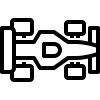
\includegraphics[width=.04\textwidth]{fig/race_car.png}};
\node at (-3.1615,6.9956) {$(x(t),y(t))$};
\end{tikzpicture}
\caption{To compute the linearized conturing error $\epsilon_c^{lin}$ and lag error $\epsilon_l^{lin}$ the track is linearized around the last solution as the estimate of the arclength progress $\hat\theta$ of the MPCC. The coordinate frame $(_Ix,_Iy)$ is the inertial reference frame the track is described in.}

\label{fig:contouring}
\end{figure}

Taking a step back we see that MPCC basically is optimizing to move the position of a virtual point given by $\theta(t)$ as far along the track as possible while steering the model of the system to keep the contouring and lag errors small. The solver than discretizes this problem and finds approximate solutions.
\section{Dynamic Model}

For now the model from \cite{liniger2015optimization} is implemented with adapted parameters. In the code the state is arranged in the following way

\begin{align}
x = \begin{bmatrix}
x\\
y\\
\phi\\
v_x\\
v_y\\
\omega\\
\theta\\
d\\
\delta
\end{bmatrix}
\end{align}
where $x$, $y$ are the position of the center of gravity, $\phi$ is the yaw angle of the car w.r.t. the world frame, $v_x$ is the longitudinal velocity, $v_y$ is the lateral velocity, $\omega$ is the yaw rate, $\theta$ the advancing parameter and lastly $d$ is the integrated motor torque and $\delta$ is the steering angle.

The input $u$ is arranged as
\begin{align}
u = \begin{bmatrix}
\dot{d}\\
\dot\theta\\
\dot\delta
\end{bmatrix}
\end{align} 

The inputs we optimize for are chosen to be the derivatives of the commandable inputs to the system such that we can penalize their smoothness.

\section{Track Parametrization}

For the track the centerline is given in waypoints. To implement MPCC we need an arclenght parametrization $\Phi$. This is realized by interpolating the waypoints using cubic bezier curves (with a cyclic boundary condition) and creating a dense lookup table with the track location and the linearization parameters. Note that in the optimization it is not practical to pass the  full bezier curve since it contains functions that the used solver has dificulties dealing with such as floor and modulo. Instead the linearization parameters are passed at every stage.   


\bibliographystyle{ieeetr}
\bibliography{sample}
\end{document}
